% Copyright 2002-2024 The University of Maryland Baltimore County (UMBC)
% 1000 Hilltop Circle, Baltimore, Maryland, 21250, USA
% https://www.csee.umbc.edu/

\documentclass[graphics]{beamer}
\usepackage{graphicx}
\usepackage{listings} % Syntax highlighing
\usepackage{fancyvrb} % Inline verbatim
\usepackage{hyperref} % Hyperlinks
\hypersetup{pdfpagemode=FullScreen}

\usepackage[normalem]{ulem}               % to striketrhourhg text
\newcommand\redout{\bgroup\markoverwith
{\textcolor{red}{\rule[0.5ex]{2pt}{0.8pt}}}\ULon}

% header in tables
\newcommand*{\thead}[1]{\multicolumn{1}{c}{\bfseries #1}}

% used for arrows from one point in the slide to another
\usepackage{tikz}
\usetikzlibrary{arrows,shapes,tikzmark}

\usetheme{Boadilla}
\title{Lecture 11: More Loops}
\author{UMBC CMSC 104}
\date{Spring 2024}

\begin{document}

\begin{frame}{}
\centering
    More Loops
\end{frame}

\frame{\tableofcontents}

\section{Loop Types}
\subsection{Counter-Controlled Repetition (Definite)}
\begin{frame}[fragile]{Counter-Controlled Repetition (Definite)}
    If it is known in advance exactly how many times a loop will execute, it is known as a \textbf{counter-controlled loop}.
    \begin{verbatim}
int i = 1;
while(i <= 10) {
    print("i = %d\n", i);
    i = i + 1;
}
    \end{verbatim}
\end{frame}

\subsection{Event-Controlled Repetition (Indefinite)}
\begin{frame}[fragile]{Event-Controlled Repetition}
    If it is \underline{not} known in advance exactly how many times a loop will execute, it is known as an \textbf{event-controlled loop}.
    \begin{verbatim}
int sum = 0, value;
printf("Enter an integer value: ");
scanf("%d", &value);
while(value != -1) {
    sum = sum + value;
    printf("Enter another value: ");
    scanf("%d", &value);
}
    \end{verbatim}
\end{frame}

\begin{frame}{Event-Controlled Repetition}
    \begin{itemize}
        \item An event-controlled loop will terminate when some \textbf{event} occurs.
        \item The event may be the occurrence of a sentinel value, as in the previous example.
        \item The are other types of events that may occur, such as reaching the end of a file, or receiving the end of the data from a network connection.
    \end{itemize}
\end{frame}

\begin{frame}[fragile]{The Three Parts of a Loop}
    \begin{lstlisting}[language=C,basicstyle=\footnotesize,keywordstyle=\color{blue},commentstyle=\color{green},showstringspaces=false,stringstyle=\color{red}]
#include<stdio.h>

int main() {
    int i = 1;  // Initialization of loop control variable
    
    /* count from 1 to 100 */
    while(i < 101) { // test of loop termination condition
        printf("%d\n", i);
        i = i + 1; // modification of loop control variable
    }
    return 0;
}
    \end{lstlisting}
\end{frame}

\subsection{for loop}
\begin{frame}[fragile]{The for Loop Repetition Structure}
    \begin{itemize}
        \item The \texttt{for} loop handles details of the counter-controlled loop automatically.
        \item The initialization of the loop control variable, the termination test condition, and control variable modification are handled in the \textbf{for} loop structure.
\begin{lstlisting}[language=C,basicstyle=\footnotesize,keywordstyle=\color{blue},commentstyle=\color{green},showstringspaces=false,stringstyle=\color{red}]
int i;
// Init.    Test.     Mod.
for(i = 1; i <= 100; i = i + 1) {
    printf("%d\n", i);
}
\end{lstlisting}
    \end{itemize}
\end{frame}

\begin{frame}{The for Loop Repetition Structure}
    \begin{itemize}
        \item Just as with a while loop, a for loop:
        \begin{itemize}
            \item initializes the loop control variable before beginning the first loop iteration,
            \item modifies the loop control variable at the very end of each iteration of the loop, and
            \item performs the loop termination test before each iteration of the loop.
        \end{itemize}
        \item The \texttt{for} loop is easier to write \& read for counter-controlled loops.
    \end{itemize}
\end{frame}

\begin{frame}[fragile]{For Examples}
    \begin{lstlisting}[language=C,basicstyle=\footnotesize,keywordstyle=\color{blue},commentstyle=\color{green},showstringspaces=false,stringstyle=\color{red}]
int i;
// Counting zero to 10
for(i = 0; i <= 10; i = i + 1) {
    printf("%d\n", i);
}

// We can go backwards too
for(i = 10; i >= 0; i = i - 1) {
    printf("%d\n", i);
}

// We can count by two's, or some other value
for(i = 0; i <= 10; i = i + 2) {
    printf("%d\n", i);
}
\end{lstlisting}
\end{frame}

\subsection{do-while loop}
\begin{frame}[fragile]{The do-while Repetition Structure}
    \begin{verbatim}
do {
    statement(s);
} while (condition);
    \end{verbatim}
    The body of a \textbf{do-while} is \underline{always} executed at least once.
    \begin{itemize}
        \item Is this true of a \texttt{while} loop?
        \item Is this true of a \texttt{for} loop?
    \end{itemize}
\end{frame}

\begin{frame}[fragile]{Example}
    \begin{lstlisting}[language=C,basicstyle=\footnotesize,keywordstyle=\color{blue},commentstyle=\color{green},showstringspaces=false,stringstyle=\color{red}]
int num;
do {
    printf("Enter a positive number: ");
    scanf("%d", &num);
    if (num <= 0) {
        printf("\nThat's not positive, try again.\n");
    }
} while(num <= 0);

// Equivalent while loop
printf("Enter a positive number: ");
scanf("%d", &num);
while(num <= 0) {
    printf("\nThat's not positive, try again.\n");
    printf("Enter a positive number: ");
    scanf("%d", &num);
}
    \end{lstlisting}
\end{frame}

\begin{frame}{do-while vs. while}
    \centering
    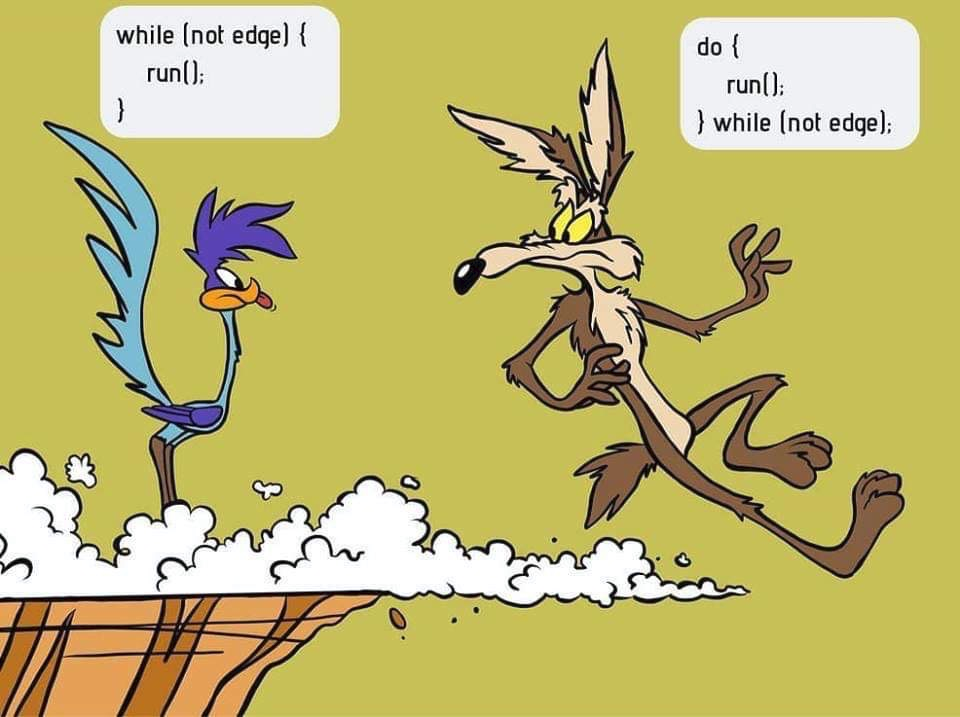
\includegraphics[scale=0.3]{L11_MoreLoops/do_while.png} \\
    \footnotesize Author unknown.
\end{frame}

\begin{frame}[fragile]{Equivalent for Loop}
    You \textit{can} use a \texttt{for} loop for an event-controlled loop, but it's rather awkward.
    \begin{lstlisting}[language=C,basicstyle=\footnotesize,keywordstyle=\color{blue},commentstyle=\color{green},showstringspaces=false,stringstyle=\color{red}]
int num;
printf("Enter a positive number: ");
scanf("%d", &num);
for(; num <= 0; ) {
    printf("\nThat's not positive, try again.\n");
    printf("Enter a positive number: ");
    scanf("%d", &num);
}
    \end{lstlisting}
\end{frame}

\section{Loop Selection}
\begin{frame}{Which Loop to Use?}
    \begin{itemize}
        \item Use a \texttt{for} loop for counter-controlled repetition.
        \item Use a \texttt{while} or \texttt{do}-\texttt{while} loop for event-controlled repetition.
        \begin{itemize}
            \item Use a \texttt{do}-\texttt{while} loop when the loop must execute at least once.
            \item Use a \texttt{while} loop when it is possible that the loop may never execute.
        \end{itemize}
    \end{itemize}
\end{frame}

\begin{frame}{Nested Loops}
    \begin{itemize}
        \item Loops may be \textbf{nested} (\textbf{embedded}) inside of each other.
        \item Any control structure (sequence, selection, repetition) may be nested inside of any other control structure, if appropriate for your algorithm.
        \item It is common to see nested for loops.
    \end{itemize}
\end{frame}

\begin{frame}[fragile]{Nested Loops}
    \begin{lstlisting}[language=C,basicstyle=\footnotesize,keywordstyle=\color{blue},commentstyle=\color{green},showstringspaces=false,stringstyle=\color{red}]
int i, j;
for ( i = 0; i < 5; i = i + 1 ) {
    for ( j = 0; j < 3; j = j + 1 ) {
        if ( j % 2 == 0 ) {
            printf("O");
        } else {
            printf("X");
        }
    }
    printf("\n");
}
    \end{lstlisting}
    \begin{itemize}
        \item How many times is the \texttt{if} statement executed?
        \item What is the output?
    \end{itemize}
\end{frame}

\section{Break \& Continue}
\begin{frame}{The break Statement}
    \begin{itemize}
        \item The \textbf{break} statement can be used in loops to cause a premature exit of the loop.
        \item Sometimes it's necessary for your algorithm to exit early, perhaps because the proper solution was found early, or because of unexpected input.
        \item Normally, it's not a recommended technique, and should only be used when needed.
    \end{itemize}
\end{frame}

\begin{frame}[fragile]{Example}
    \begin{lstlisting}[language=C,basicstyle=\footnotesize,keywordstyle=\color{blue},commentstyle=\color{green},showstringspaces=false,stringstyle=\color{red}]
#include <stdio.h>
int main() {
    int i;
    for(i = 1; i < 10; i++) {
        if (i == 5) {
            break;
        }
        printf("%d ", i);
    }
    printf("Broke out of loop at i = %d\n", i);
    return 0;
}
    \end{lstlisting}
    Output:
    \begin{verbatim}
1 2 3 4
Broke out of loop at i = 5
    \end{verbatim}
\end{frame}

\begin{frame}{The continue Statement}
    \begin{itemize}
        \item The \textbf{continue} statement can be used in loops to skip computation for that particular iteration.
        \item Sometimes it's necessary for your algorithm to skip an iteration, perhaps to avoid an error.
        \item Normally, it's not a recommended technique, and should only be used when needed.
    \end{itemize}
\end{frame}

\begin{frame}[fragile]{Example}
    \begin{lstlisting}[language=C,basicstyle=\footnotesize,keywordstyle=\color{blue},commentstyle=\color{green},showstringspaces=false,stringstyle=\color{red}]
#include <stdio.h>
int main() {
    int i;
    for(i = 1; i < 10; i++) {
        if (i == 5) {
            continue;
        }
        printf("%d ", i);
    }
    printf("\nDone\n");
    return 0;
}
    \end{lstlisting}
    Output:
    \begin{verbatim}
1 2 3 4 6 7 8 9

Done
    \end{verbatim}
\end{frame}

\end{document}